\documentclass[12pt, a4paper]{article}

% --- Packages for Aesthetics ---
\usepackage[utf8]{inputenc}
\usepackage[margin=2cm]{geometry}
\usepackage{xcolor}
\usepackage{tcolorbox}
\usepackage{titlesec}
\usepackage{enumitem}
\usepackage{fourier} % Modern font
\usepackage{booktabs}
\usepackage{tabularx}
\usepackage{colortbl}
\usepackage{multirow}
\usepackage{tikz}
\usetikzlibrary{shapes.geometric, arrows, positioning, shadows, patterns}

% --- Color Palette ---
\definecolor{primary}{HTML}{2D3436}
\definecolor{accent}{HTML}{0984E3}
\definecolor{softblue}{HTML}{74B9FF}
\definecolor{lightgray}{HTML}{F5F6FA}
\definecolor{tableheader}{HTML}{dfe6e9}
\definecolor{nature}{HTML}{00b894}
\definecolor{love}{HTML}{d63031}
\definecolor{dark}{HTML}{2d3436}
\definecolor{science}{HTML}{0984e3}

% --- Custom Box Styles ---
\tcbset{
    sharp corners,
    boxrule=0.5pt,
    colback=white,
    colframe=primary,
    fonttitle=\bfseries,
    colbacktitle=accent,
    coltitle=white,
    enhanced,
    attach boxed title to top left={yshift=-2mm, xshift=2mm},
    boxed title style={sharp corners}
}

% --- Title Styling ---
\titleformat{\section}{\color{accent}\Large\bfseries}{}{0em}{}[\titlerule]
\titleformat{\subsection}{\color{primary}\large\bfseries}{}{0em}{}

\begin{document}

% ==========================================
% PAGE 1: TITLE & PROBLEM STATEMENT
% ==========================================
\begin{center}
    \vspace*{2cm}
    {\Huge \bfseries \color{primary} Symphony of Words} \\
    \vspace{0.5cm}
    {\Large \bfseries A Hybrid Architecture for Autonomous Poetry Generation} \\
    \vspace{1cm}
    \begin{tcolorbox}[colback=lightgray, colframe=accent, width=0.6\textwidth, center title]
        \centering
        \textbf{Authors:} \\
        Maria-Daria Tompea \\
        İlayda Tiryaki \\
        \vspace{0.2cm}
        \textbf{Deadline:} May 18, 2026
    \end{tcolorbox}
    \vspace{2cm}
\end{center}

\section{1. Problem Statement: The Goal}
\begin{tcolorbox}[title=What is Poetry Generation?]
Poetry generation is the task of making a computer write verses that sound human. It's not just about picking words; it's about making them feel "right."
\end{tcolorbox}

Writing a poem is hard for a machine because it has to balance four main things:
\begin{enumerate}
    \item \textbf{Syntax:} The poem must follow basic grammar rules.
    \item \textbf{Semantics:} It should stay on a specific topic (if the user wants a poem about "stars", it shouldn't talk about "sandwiches").
    \item \textbf{Aesthetics:} It needs to have rhythm, maybe some rhyme, and "fancy" poetic words.
    \item \textbf{Creativity:} It shouldn't just copy-paste from a book. It needs to create something new.
\end{enumerate}

\begin{center}
    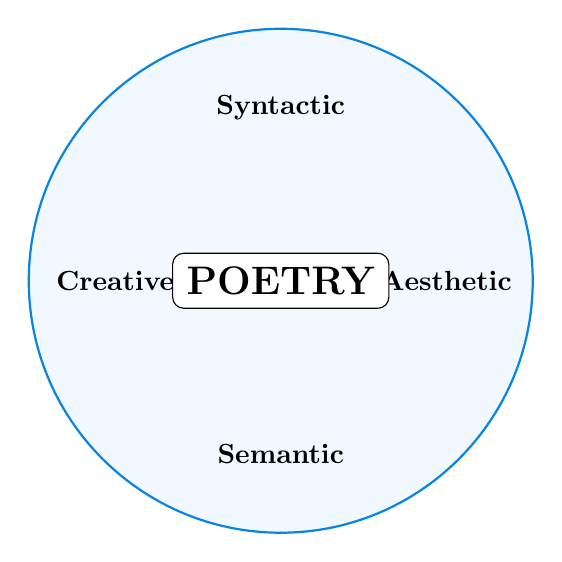
\begin{tikzpicture}
        \draw[fill=softblue!10, draw=accent, thick] (0,0) circle (3.2cm);
        \node[font=\bfseries] at (0,2.2) {Syntactic};
        \node[font=\bfseries] at (0,-2.2) {Semantic};
        \node[font=\bfseries] at (2.1,0) {Aesthetic};
        \node[font=\bfseries] at (-2.1,0) {Creative};
        \node[draw, fill=white, rounded corners, inner sep=5pt, font=\Large\bfseries] at (0,0) {POETRY};
    \end{tikzpicture}
    \small \\ \textit{Figure 1: The four pillars of computational poetry.}
\end{center}

\newpage

% ==========================================
% PAGE 2: PROPOSED SOLUTION - MARKOV
% ==========================================
\section{2. Proposed Solution: Two Creative Paths}
Our system uses two different ways to generate text. We call them the \textbf{Stochastic Path} and the \textbf{Creative Path}.

\subsection{2.1 The Stochastic Path (Markov Chains)}
This is the "pattern-matching" engine. It works like the predictive text on your phone but much smarter. It looks at our 2,000-line corpus and calculates which words usually come after each other.

\begin{tcolorbox}[title=How it predicts words]
If the AI sees the words \textbf{"The silent"}, it checks its table and finds:
\begin{itemize}
    \item \textbf{night} (40\% chance)
    \item \textbf{darkness} (30\% chance)
    \item \textbf{shadow} (20\% chance)
\end{itemize}
It then picks one based on these probabilities.
\end{tcolorbox}

\begin{center}
    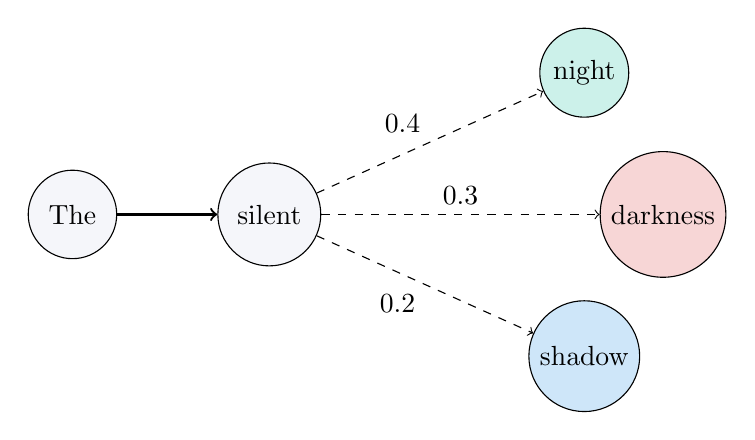
\begin{tikzpicture}[node distance=2.5cm, auto]
        \node (w1) [circle, draw, fill=lightgray, inner sep=5pt] {The};
        \node (w2) [circle, draw, fill=lightgray, right of=w1, inner sep=5pt] {silent};
        \node (w3) [circle, draw, fill=nature!20, right of=w2, yshift=1.8cm, xshift=1.5cm, inner sep=3pt] {night};
        \node (w4) [circle, draw, fill=love!20, right of=w2, yshift=0cm, xshift=2.5cm, inner sep=3pt] {darkness};
        \node (w5) [circle, draw, fill=science!20, right of=w2, yshift=-1.8cm, xshift=1.5cm, inner sep=3pt] {shadow};
        
        \draw [->, thick] (w1) -- (w2);
        \draw [->, dashed] (w2) -- node[above left] {0.4} (w3);
        \draw [->, dashed] (w2) -- node[above] {0.3} (w4);
        \draw [->, dashed] (w2) -- node[below left] {0.2} (w5);
    \end{tikzpicture}
    \small \\ \textit{Figure 2: A simple Markov Transition Graph.}
\end{center}

\subsection{Advantages of this path:}
\begin{itemize}
    \item It is very fast (instant generation).
    \item It creates surprising and "dreamy" word combinations.
\end{itemize}

\newpage

% ==========================================
% PAGE 3: PROPOSED SOLUTION - CR-PO & FACE
% ==========================================
\subsection{2.2 The Creative Path (CR-PO \& Full-FACE)}
This is the "Advanced" engine. It doesn't just guess words; it builds them based on a plan.

\begin{enumerate}
    \item \textbf{CR-PO (Constrained Recombination):} The system checks every word in a draft. If a word is "boring" (like "car"), it replaces it with something related to the theme (like "chariot").
    \item \textbf{Full-FACE Model:} This model makes the AI \textit{think} about what it's doing.
    \begin{itemize}
        \item \textbf{Concepts:} Picking a template (e.g., AABB rhyme scheme).
        \item \textbf{Aesthetics:} Evaluating if the poem sounds "happy" or "sad".
        \item \textbf{Framing:} Writing a commentary to explain the poem.
    \end{itemize}
\end{enumerate}

\begin{center}
    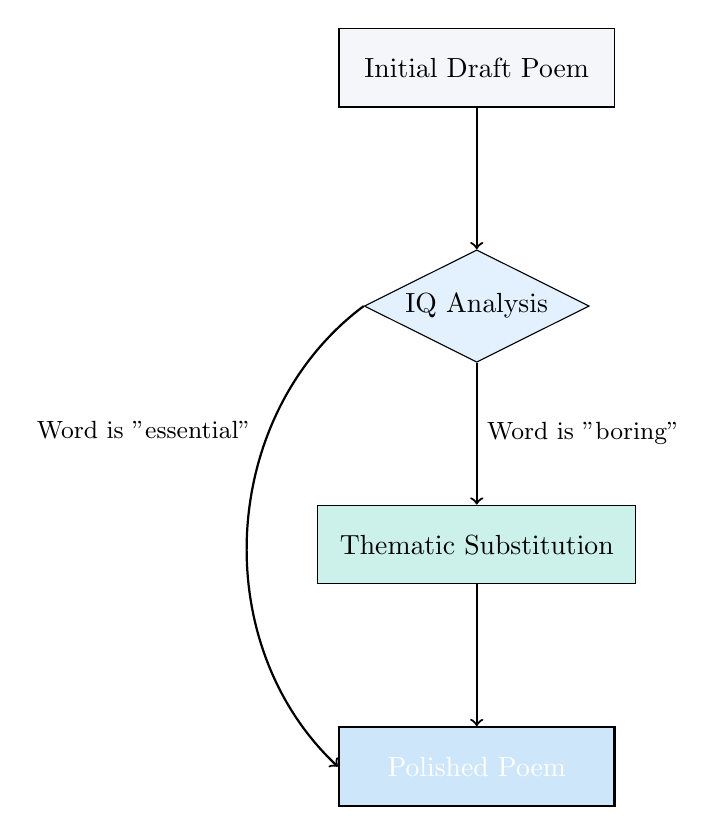
\begin{tikzpicture}[node distance=1.8cm and 2cm, block/.style={rectangle, draw, minimum height=1cm, minimum width=3.5cm, inner sep=8pt}]
        \node (draft) [block, fill=lightgray] {Initial Draft Poem};
        \node (iq) [diamond, draw, below=of draft, aspect=2, fill=softblue!20, inner sep=2pt] {IQ Analysis};
        \node (sub) [block, below=of iq, fill=nature!20] {Thematic Substitution};
        \node (final) [block, below=of sub, fill=accent!20, text=white, thick] {Polished Poem};
        
        \draw [->, thick] (draft) -- (iq);
        \draw [->, thick] (iq) -- node[right, font=\small] {Word is "boring"} (sub);
        \draw [->, thick] (sub) -- (final);
        \draw [->, thick, bend right=50] (iq.west) to node[left, pos=0.3, xshift=-0.1cm, font=\small] {Word is "essential"} (final.west);
    \end{tikzpicture}
    \small \\ \textit{Figure 3: The CR-PO Refinement Funnel.}
\end{center}

\begin{tcolorbox}[title=The FACE Model Cycle, colback=accent!5, colframe=accent]
    \centering
    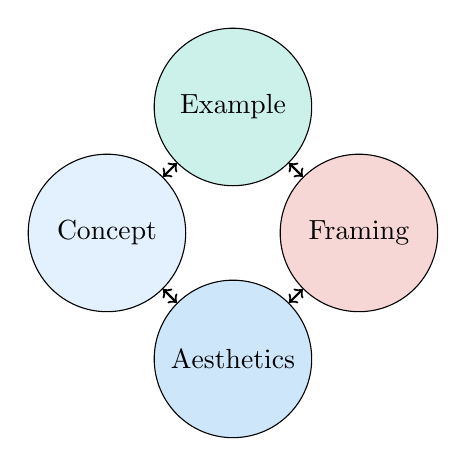
\begin{tikzpicture}[scale=0.8]
        \node[draw, circle, minimum size=2cm, fill=nature!20] (E) at (0,2) {Example};
        \node[draw, circle, minimum size=2cm, fill=love!20] (F) at (2,0) {Framing};
        \node[draw, circle, minimum size=2cm, fill=science!20] (A) at (0,-2) {Aesthetics};
        \node[draw, circle, minimum size=2cm, fill=softblue!20] (C) at (-2,0) {Concept};
        \draw[<->, thick] (E) -- (F); \draw[<->, thick] (F) -- (A);
        \draw[<->, thick] (A) -- (C); \draw[<->, thick] (C) -- (E);
    \end{tikzpicture}
\end{tcolorbox}

\newpage

% ==========================================
% PAGE 4: DATA SET ANALYSIS
% ==========================================
\section{3. Data Set Analysis: What the AI Learned}
We didn't just give the AI any text; we gave it a curated "library" of over 2,000 lines of poetry.

\begin{tcolorbox}[title=Corpus Composition]
\renewcommand{\arraystretch}{1.2}
\rowcolors{2}{lightgray!50}{white}
\begin{tabularx}{\textwidth}{l X l r}
    \rowcolor{tableheader} \textbf{Genre} & \textbf{Style} & \textbf{Source} & \textbf{Weight} \\
    \midrule
    Romantic & Nature & Wordsworth, Keats & 35\% \\
    Shakespearean & Love & Sonnets 1-154 & 25\% \\
    Symbolist & Dark/Deep & Baudelaire, Verlaine & 20\% \\
    Science & Modern & Original Verses & 20\% \\
    \bottomrule
\end{tabularx}
\end{tcolorbox}

\begin{center}
    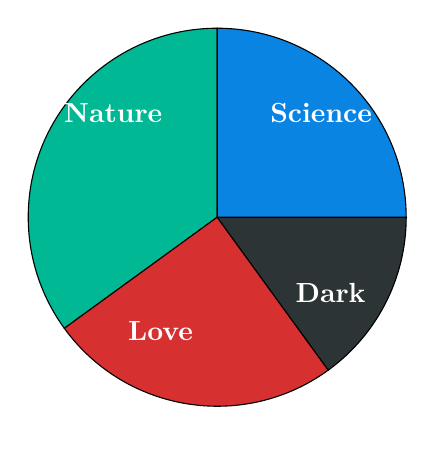
\begin{tikzpicture}[scale=1.2]
        % Pie Chart with better labels
        \draw[fill=nature] (0,0) -- (0,2) arc (90:216:2cm) -- cycle; % 35%
        \draw[fill=love] (0,0) -- (-1.618,-1.176) arc (216:306:2cm) -- cycle; % 25%
        \draw[fill=dark] (0,0) -- (1.176,-1.618) arc (306:360:2cm) -- cycle; % 15%
        \draw[fill=science] (0,0) -- (2,0) arc (0:90:2cm) -- cycle; % 25%
        
        \node at (-1.1, 1.1) {\color{white}\textbf{Nature}};
        \node at (-0.6, -1.2) {\color{white}\textbf{Love}};
        \node at (1.2, -0.8) {\color{white}\textbf{Dark}};
        \node at (1.1, 1.1) {\color{white}\textbf{Science}};
    \end{tikzpicture}
    \small \\ \textit{Figure 4: Distribution of the training corpus by genre.}
\end{center}

\subsection{Top Poetic Keywords}
Our analysis shows the most frequent words the AI uses to stay on theme:
\begin{center}
    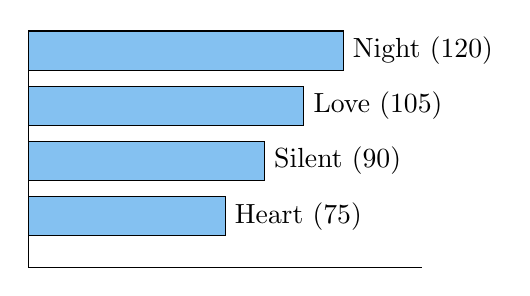
\begin{tikzpicture}
        \draw[fill=accent!50] (0,0) rectangle (4,0.5); \node[right] at (4,0.25) {Night (120)};
        \draw[fill=accent!50] (0,-0.7) rectangle (3.5,-0.2); \node[right] at (3.5,-0.45) {Love (105)};
        \draw[fill=accent!50] (0,-1.4) rectangle (3,-0.9); \node[right] at (3,-1.15) {Silent (90)};
        \draw[fill=accent!50] (0,-2.1) rectangle (2.5,-1.6); \node[right] at (2.5,-1.85) {Heart (75)};
        \draw (0,0) -- (0,-2.5) -- (5,-2.5);
    \end{tikzpicture}
\end{center}

\newpage

% ==========================================
% PAGE 5: SYSTEM ARCHITECTURE
% ==========================================
\section{4. System Architecture: The Design}
The application is designed to be user-friendly while having a very complex backend.

\begin{center}
    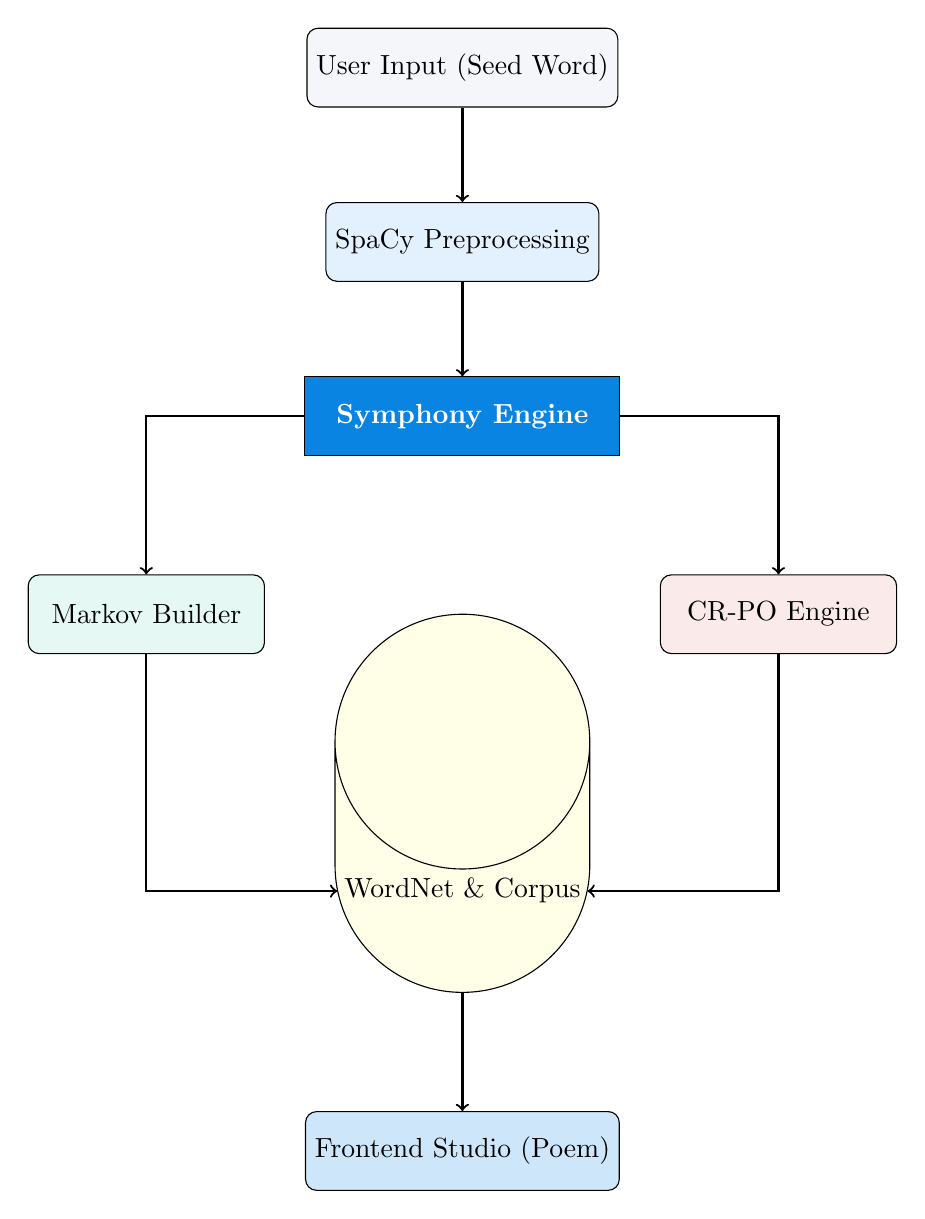
\begin{tikzpicture}[
        node distance=1.2cm and 1cm,
        block/.style={rectangle, draw, fill=lightgray!20, text centered, rounded corners, minimum height=1cm, minimum width=3cm},
        engine/.style={rectangle, draw, fill=accent, text=white, font=\bfseries, text centered, minimum height=1cm, minimum width=4cm},
        database/.style={cylinder, draw, shape border rotate=90, fill=yellow!10, minimum height=1.5cm, minimum width=2cm, text centered}
    ]
        % Nodes
        \node (in) [block, fill=lightgray] {User Input (Seed Word)};
        \node (pre) [block, below=of in, fill=softblue!20] {SpaCy Preprocessing};
        \node (eng) [engine, below=of pre] {Symphony Engine};
        
        \node (m1) [block, below left=1.5cm and 0.5cm of eng, fill=nature!10] {Markov Builder};
        \node (m2) [block, below right=1.5cm and 0.5cm of eng, fill=love!10] {CR-PO Engine};
        
        \node (db) [database, below=2cm of eng] {WordNet \& Corpus};
        \node (out) [block, below=1.5cm of db, fill=accent!20] {Frontend Studio (Poem)};
        
        % Arrows
        \draw [->, thick] (in) -- (pre);
        \draw [->, thick] (pre) -- (eng);
        
        \draw [->, thick] (eng) -| (m1);
        \draw [->, thick] (eng) -| (m2);
        
        \draw [->, thick] (m1) |- (db);
        \draw [->, thick] (m2) |- (db);
        \draw [->, thick] (db) -- (out);
    \end{tikzpicture}
    \small \\ \textit{Figure 5: Full Application Diagram.}
\end{center}

\begin{tcolorbox}[title=How it works step-by-step]
\begin{enumerate}
    \item \textbf{Input:} You type a word like "Space".
    \item \textbf{Preprocessing:} The AI learns that "Space" is a NOUN.
    \item \textbf{Generation:} It picks a path. Markov makes a fast draft. CR-PO makes a precise, rhyming draft.
    \item \textbf{Refinement:} WordNet swaps words like "stars" with "celestial lights".
    \item \textbf{Display:} You see the final poem in the "Symphony Studio" web interface.
\end{enumerate}
\end{tcolorbox}

\newpage

% ==========================================
% PAGE 6: IMPLEMENTATION & RESULTS
% ==========================================
\section{5. Implementation Details}
We used modern tools to make this possible:
\begin{itemize}
    \item \textbf{Python (Backend):} The "brains" of the operation.
    \item \textbf{SpaCy:} Used for understanding grammar and parts of speech.
    \item \textbf{WordNet:} A huge database of synonyms we use for lexical substitution.
    \item \textbf{FastAPI:} Connects the Python code to the website.
    \item \textbf{JavaScript (Frontend):} Creates the "Symphony Studio" interface.
\end{itemize}

\section{6. Experiments and Results}
We compared both pathways to see which one works better.

\begin{tcolorbox}[title=Final Comparison Table]
\renewcommand{\arraystretch}{1.5}
\begin{tabularx}{\textwidth}{l X X}
    \rowcolor{tableheader} \textbf{Feature} & \textbf{Markov Path} & \textbf{CR-PO Path} \\
    \midrule
    \textbf{Speed} & Instant (Fast) & 2-3 Seconds (Slow) \\
    \textbf{Grammar} & Medium & Very High \\
    \textbf{Rhyme/Meter} & Random & Guaranteed \\
    \textbf{Best For} & Inspiration & Finished Poems \\
    \bottomrule
\end{tabularx}
\end{tcolorbox}

\subsection{Conclusion}
The **Markov Path** is great when you want something fast and abstract. The **CR-PO Path** is better when you want a professional-sounding poem that follows strict rules. By combining both, **Symphony of Words** gives the user total control over their creative process.

\begin{center}
    \vspace{2cm}
    \color{accent} \Huge \textbf{Thank You!}
\end{center}

\end{document}
